%!TEX root = ClementiBarba2020.tex

\subsection{Replication of results from Rockstuhl, et al., 2005}

%%% Rockstuhl work summary%%%%
The work of Rockstuhl et al.\cite{rockstuhl2005} study the phonon-polariton response of silicon carbide (SiC)
nanoparticles using the boundary element method. They analyze different "cylindrical particles"
made of 6H-SiC as a function of geometrical cross section. These "cylinders" have an infinite
extension in the third dimension, and they solve these geometries numerically with a 2D 
boundary element method from their previous work \cite{rockstuhl2003}. 
%%% Rockstuhl work summary%%%%


We decided to replicate one of the results that they present on Fig.14 of their paper, which 
presents the scattering cross section of a SiC rectangular cylinder for three different object 
sizes. To complain with our quasistatic approach ($\lambda > d$ where $d$) we chose the particular 
case where a=672 nm and b=328 nm.

\textbf{Difference between methods, mesh and dielectric data}

\textit{method}: The main difference between Rockstuhl simulations and ours is that they solve a 2D problem, 
while we solve a 3D model. In our case the geometry has a finite third dimension. To cope with this
we will extend the third direction considerably, and study this effect.
We compute extinction cross section (scattering plus absorption) while Rockstuhl work present only scattering. 
But since in both scattering and absorption the resonance occur at the same wavelengths, the results are 
comparable.

\textit{mesh}: Their work does not provide any details regarding the discretization of their geometries or 
parameters involved in the simulations. We performed a grid independence study to make sure that we are
solving properly the physics and minimizing errors due to discretization. 

\textit{dielectric data}: The use 6H-SiC as material, and they obtained their data from a a source that we
were not able to replicate. Instead we are using experimental data for 4h-SiC that was provided to us 
via private communications.  

\subsubsection{Grid independance study}

We performed a grid independence study on a SiC cube of side $L=535$ nm submerged in air, under a 
constant electric field aligned with the z-axis.
(similar to quadratic cylinder on Fig 18 of Rockstuhl et.al). 
Due to the nature of the geometry, and its sharp edges it was challenging to see proper convergence. However,
for this type of physics, convergence has been studied in our previous work \cite{ClementiCooperBarba2019}. 
In the Figure \ref{fig:cube535} we show a grid independence study, where we go from a mesh of 15552 
triangles (density = 1.11x10$^-4$ $N/\text{\AA}$) to 19200 (density = 9.05x10$^-5$ $N/\text{\AA}$) 
triangles and the computed results do not change.

\begin{figure}
    \centering
    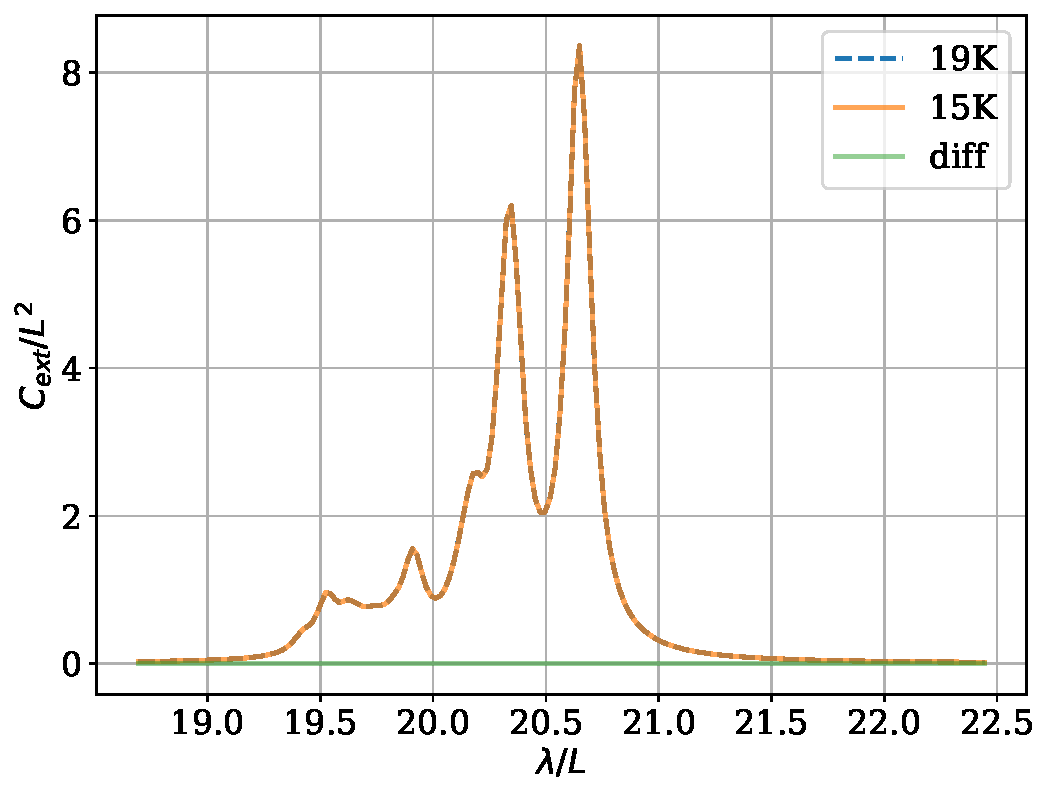
\includegraphics[width=0.85\textwidth]{cubeL535nm_15Kvs19K.pdf} 
    \caption{Grid independence study for a SiC cube of side $L=535 nm$ submerged in air under a constant 
    electric field in the z-direction. The curves represent the extinction cross section divided by $L^2$ 
    as a function of wavelength divided by $L$}
    \label{fig:cube535}
 \end{figure}

It is worth noting that the extinction cross section curve in Figure \ref{fig:cube535} has extra peaks, 
compared to the results of Figure 18 on Rockstuhl, this is due to the 3D nature of our case and the sharp 
edges. This will be approach in the following results where we attempt a replication of one of teh results 
of Figure 14 of Rockstuhl work.

\subsubsection{Replication of Figure 14 (case a1) of Rockstuhl 2005}

Based on the reuslts of the grid independence stud we decided to we used the density of the cube as a reference to produce the meshes for the replication 
of figures 14a and 14b on Rockstuhl's work (case a1=672, b=328). This simulation is a "rectangular cylinder" of 
dimensions (we chose a case that will go well with our quasistatic model) are $a=672$ nm and $b=328$ nm. 

Effect of extended third dimension (in our case this is the y axis) are in Figures \ref{fig:ext_y_14} and


\begin{figure}
    \centering
    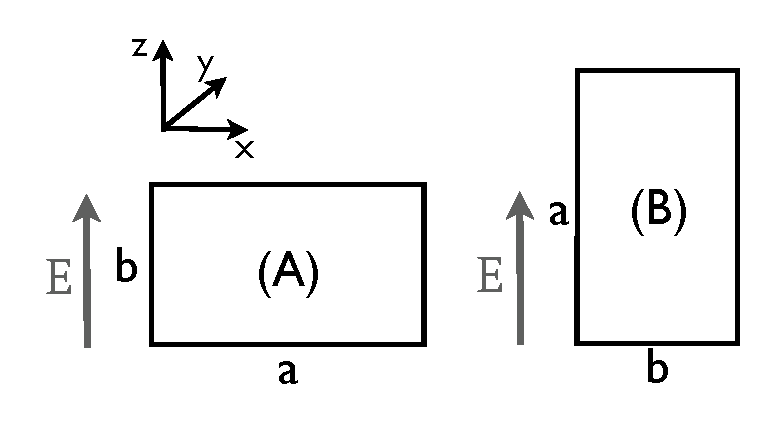
\includegraphics[width=0.45\textwidth]{rockstuhl_rectangles.pdf} 
    \caption{Rockstuhl runs configurations}
    \label{fig:rectangle_sketch}
\end{figure}

\begin{figure}
    \centering
    \subfloat{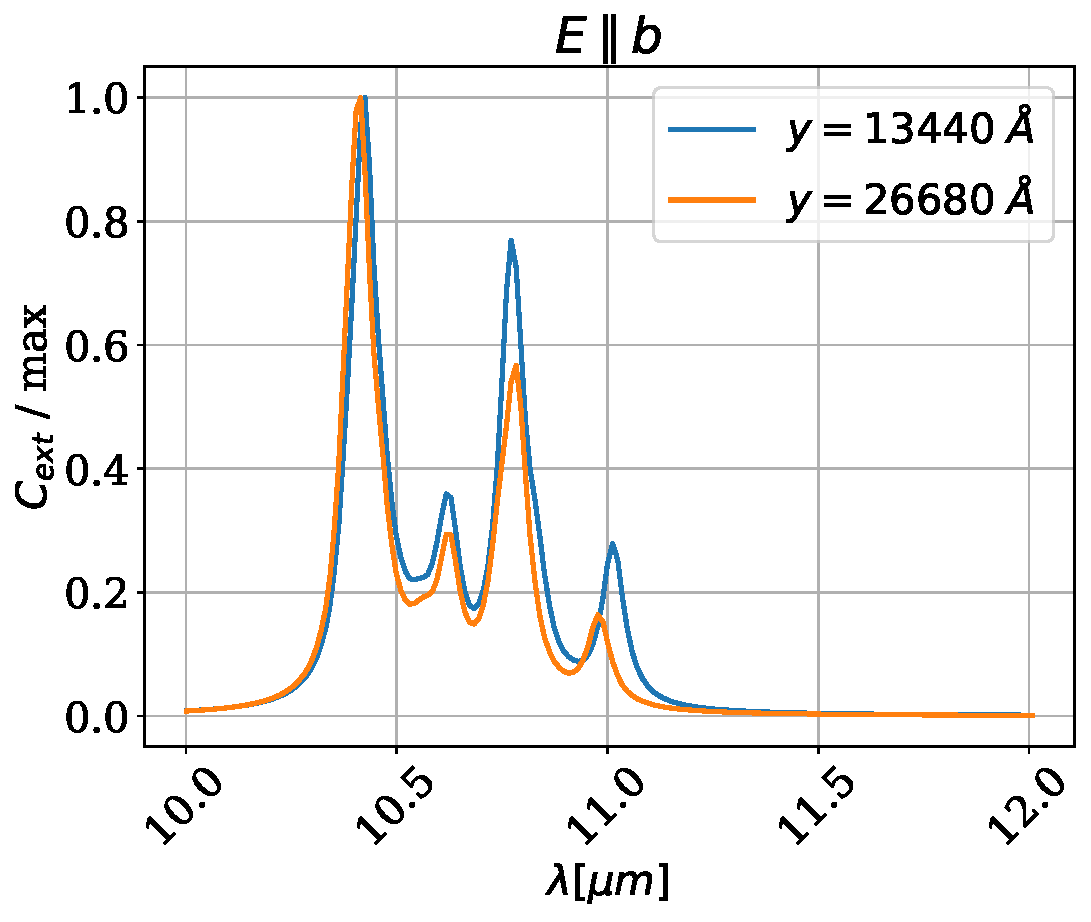
\includegraphics[width=0.45\textwidth]{ext_y_14a.pdf}}
    \subfloat{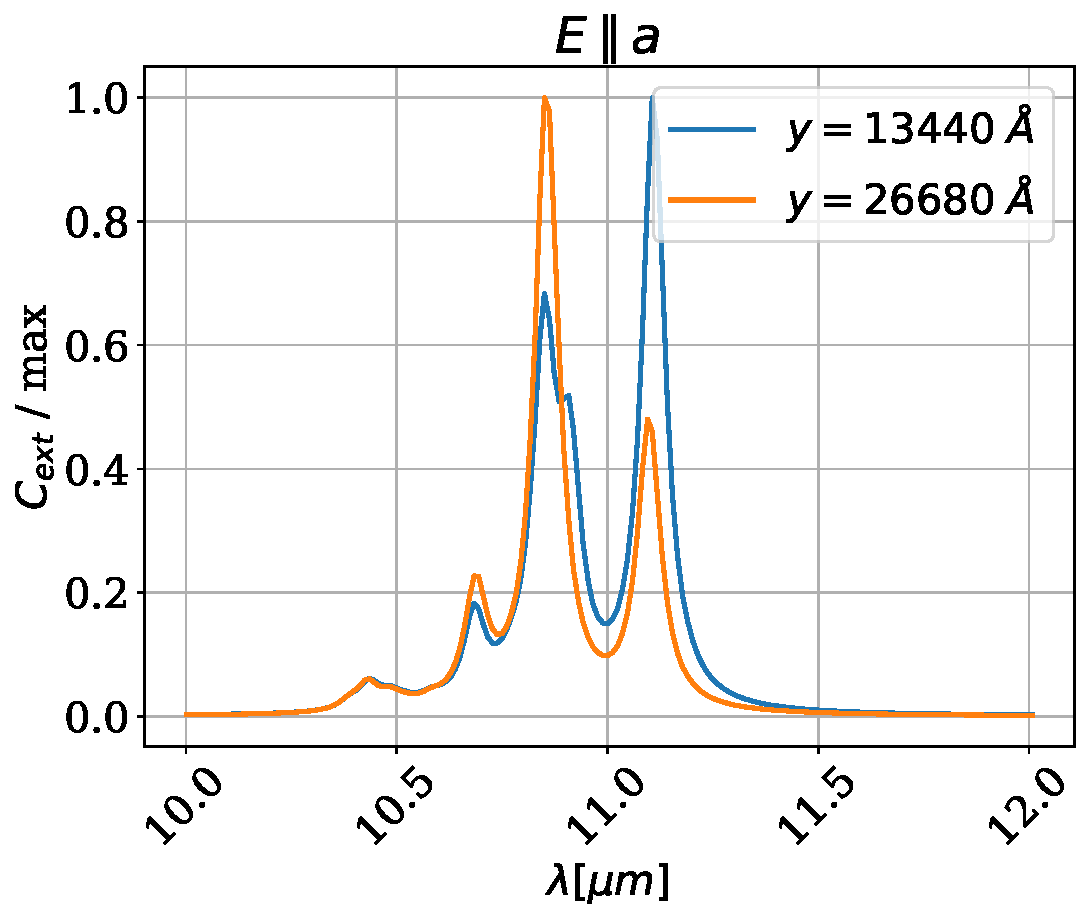
\includegraphics[width=0.45\textwidth]{ext_y_14b.pdf}} 
    %\caption{Extension of third dimension (y-axis) study for the case of rectangle prism of dimensions a=672 nm and b= 328 nm.
    %        Attempt of replication of Figure 14 a on Rockstuhl paper (case a1). In this case we have the constant 
    %        electric field parallel to the short dimension (b), and the geometry is in air. 
    %        Normalized (by max) Extinction cross section of a rectangle for two different y-values in the 
    %        short edge configuration (electric field parallel to the shorter dimension)}
    %\label{fig:ext_y_14a}
    %\label{fig:ext_y_14b}
    \caption{THIS IS A BIG CAPTION}
    \label{fig:ext_y_14}   
 \end{figure}


We see that as we elongate the third dimension the extra peaks start fading. 

At this point we noticed that the mesher (trimesh) was not generating a uniform mesh. We created our 
own mesher, and tested the difference. Moreover, the paper mentioned that they rounded the corners of their
"rectangular cylinder". We were able to give our mesh as input to trimesh and round the edges but we were not able 
to know how the roundness was related to the arc of the curvature. This were parameters with no physical meaning, 
therefore we decided to go with the default setting. 


\begin{figure}
    \centering
    \subfloat{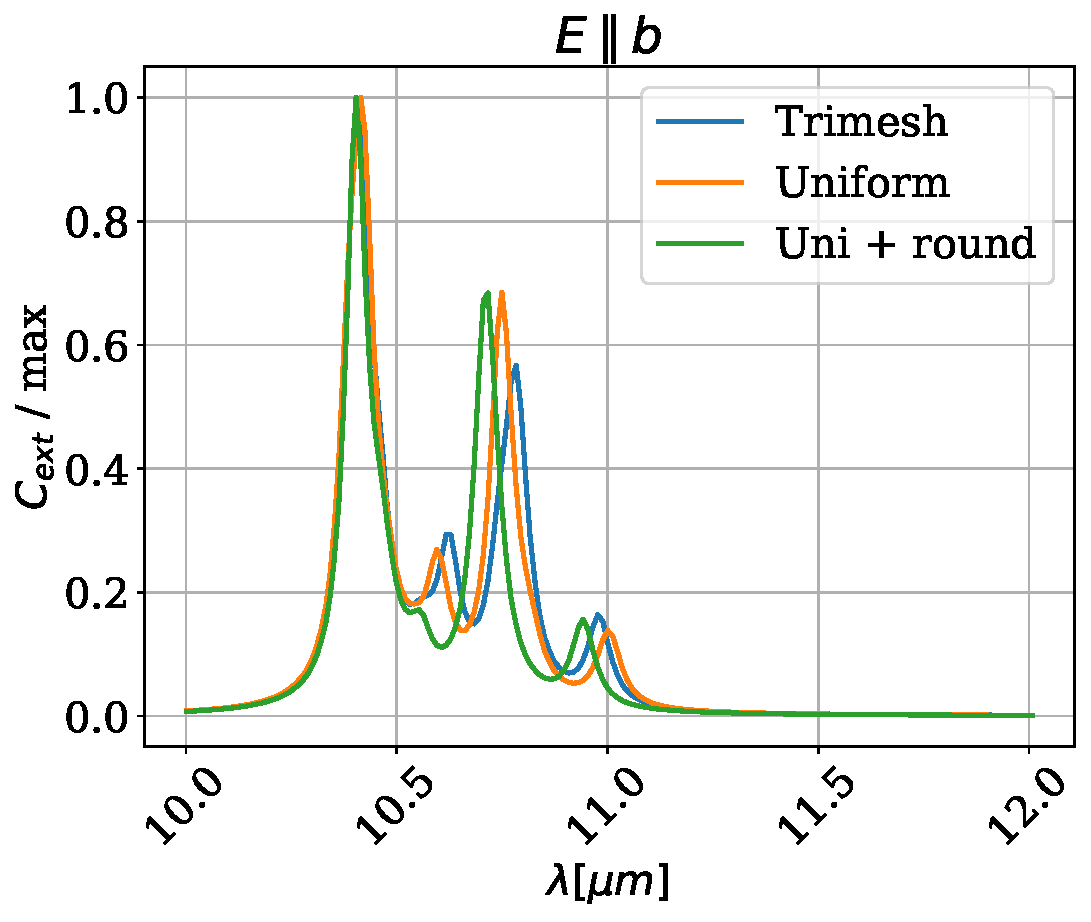
\includegraphics[width=0.45\textwidth]{tri_reg_round_14a.pdf}}
    \subfloat{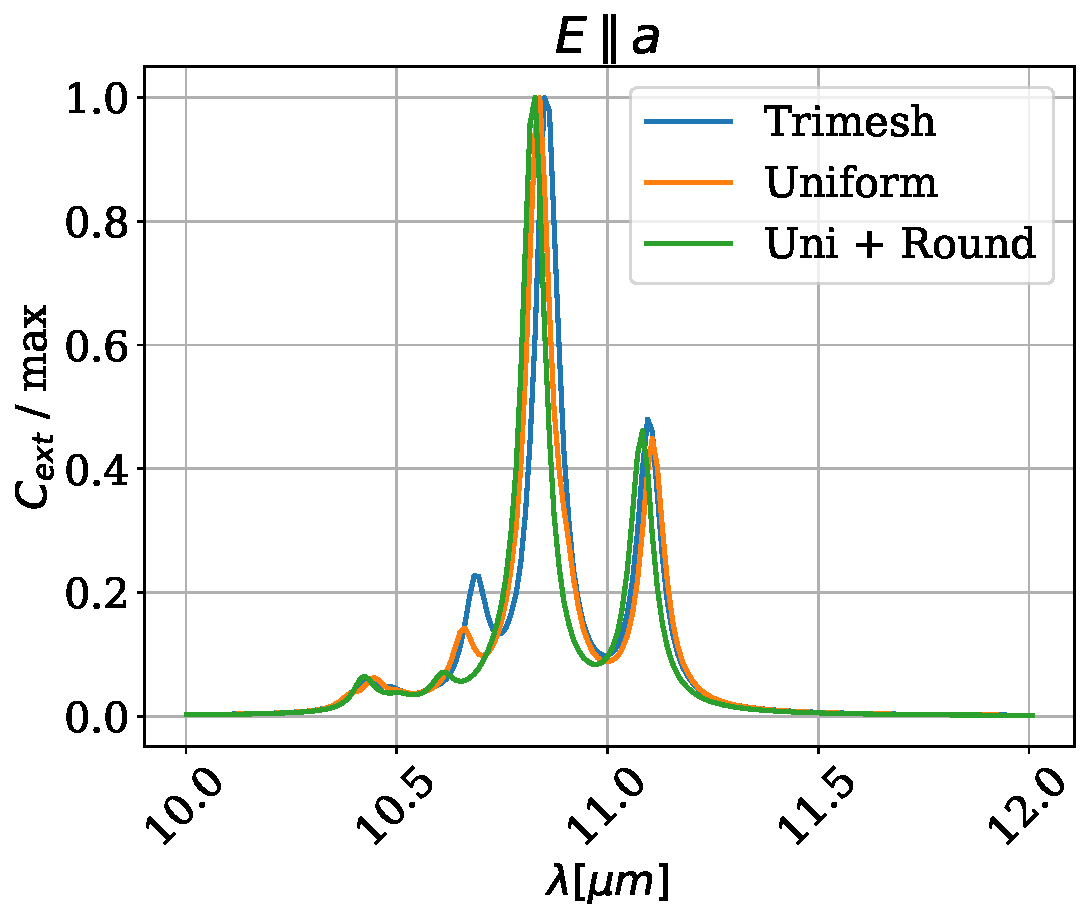
\includegraphics[width=0.45\textwidth]{tri_reg_round_14b.pdf}}
    \caption{Normalized (by max) Extinction cross section of a rectangle. Original trimesh, regular, and regular with 
    roundness. Short edge configuration (electric field parallel to the shorter (left) dimension)}
    \label{fig:tri_reg_round_14}
 \end{figure}


 Finally with all this info, here is the replication of Figures 14a and 14b. 

 \begin{figure}
    \centering
    \subfloat{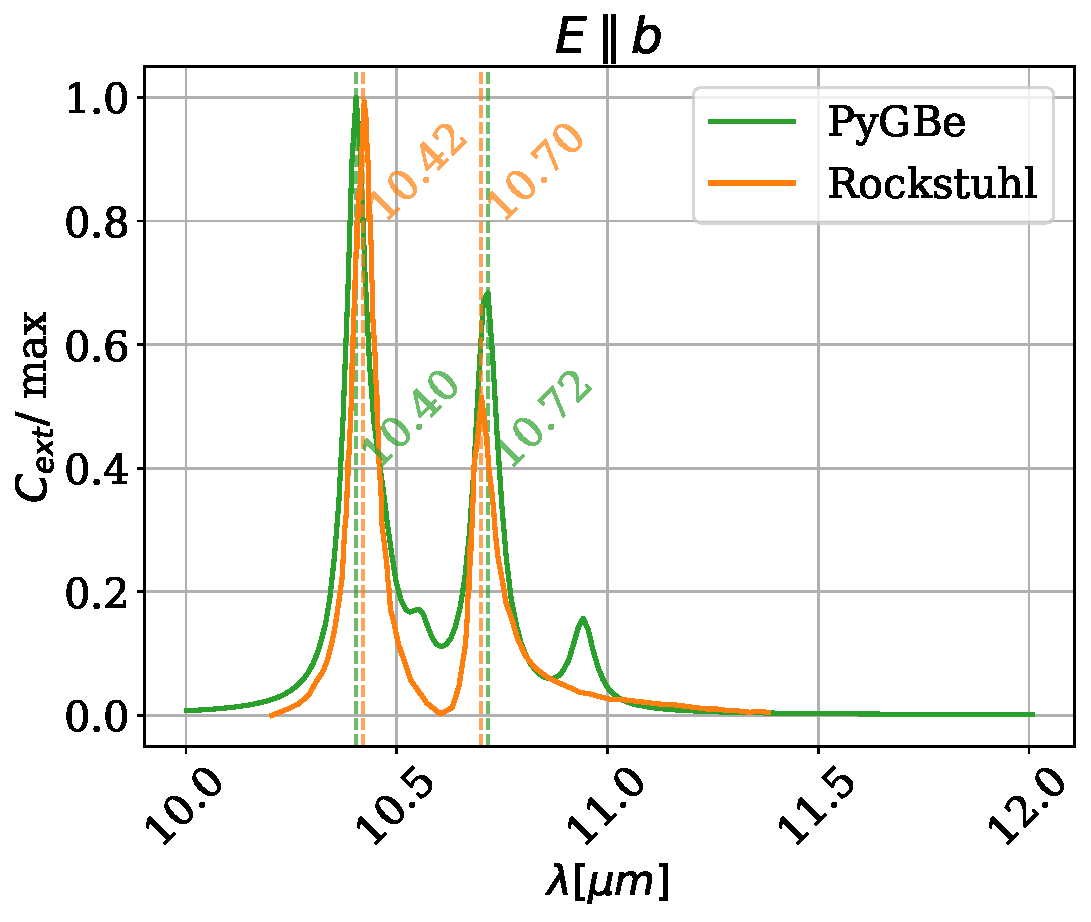
\includegraphics[width=0.45\textwidth]{replication_14a.pdf}}
    \subfloat{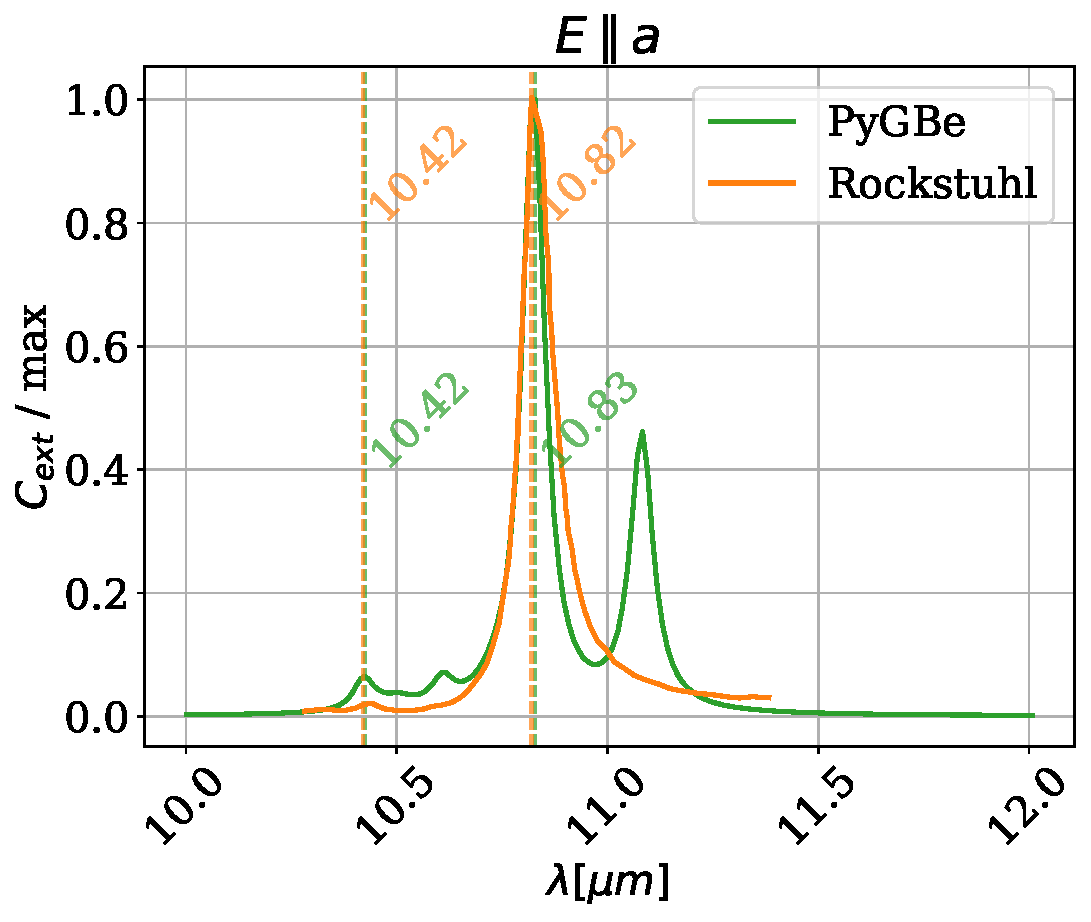
\includegraphics[width=0.45\textwidth]{replication_14b.pdf}} 

    \caption{Normalized (by max) Extinction cross section of a rectangle. Replication of 
    the short (long) edge configuration (electric field parallel to the shorter (longer) dimension)}
    \label{fig:rep_14}
 \end{figure}


 \subsection{Replication of results from Ellis et al., 2016, and validation}

There are two results from this paper that we aim to replicate, and one of them is a comparison
against experimental results which will lead to a validation. 

The first result we show is a replication of a result presented in their supplementary 
material FigureS4 {\color{red}(note sure how to cite this, maybe a link)}. We aimed to replicate the 
black curve since the simulation setup is possible to replicate using PyGBe. For each aspect ratio (AR) 
value from 1 to 7 we computed the extinction cross section $C_{ext}$ across the wave number in the range
800-1000 $cm^{-1}$, we identify the the lower frequency mode ($E_{100}$ in Ellis paper)  that is not a 
longitudinal mode. We identify the Longitudinal modes by comparing normal vs 22 deg incidence runs. These
modes due to its nature do not show up in the normal incidence runs. Then, on the 22 deg incidence 
computations we choose the lower wave number mode that it's not a longitudinal mode. The simulations were 
performed for the Long Edge orientation, meaning that the electric field is polarized along the long edge 
of the pillar that is not the height. 

\begin{figure}
    \centering
    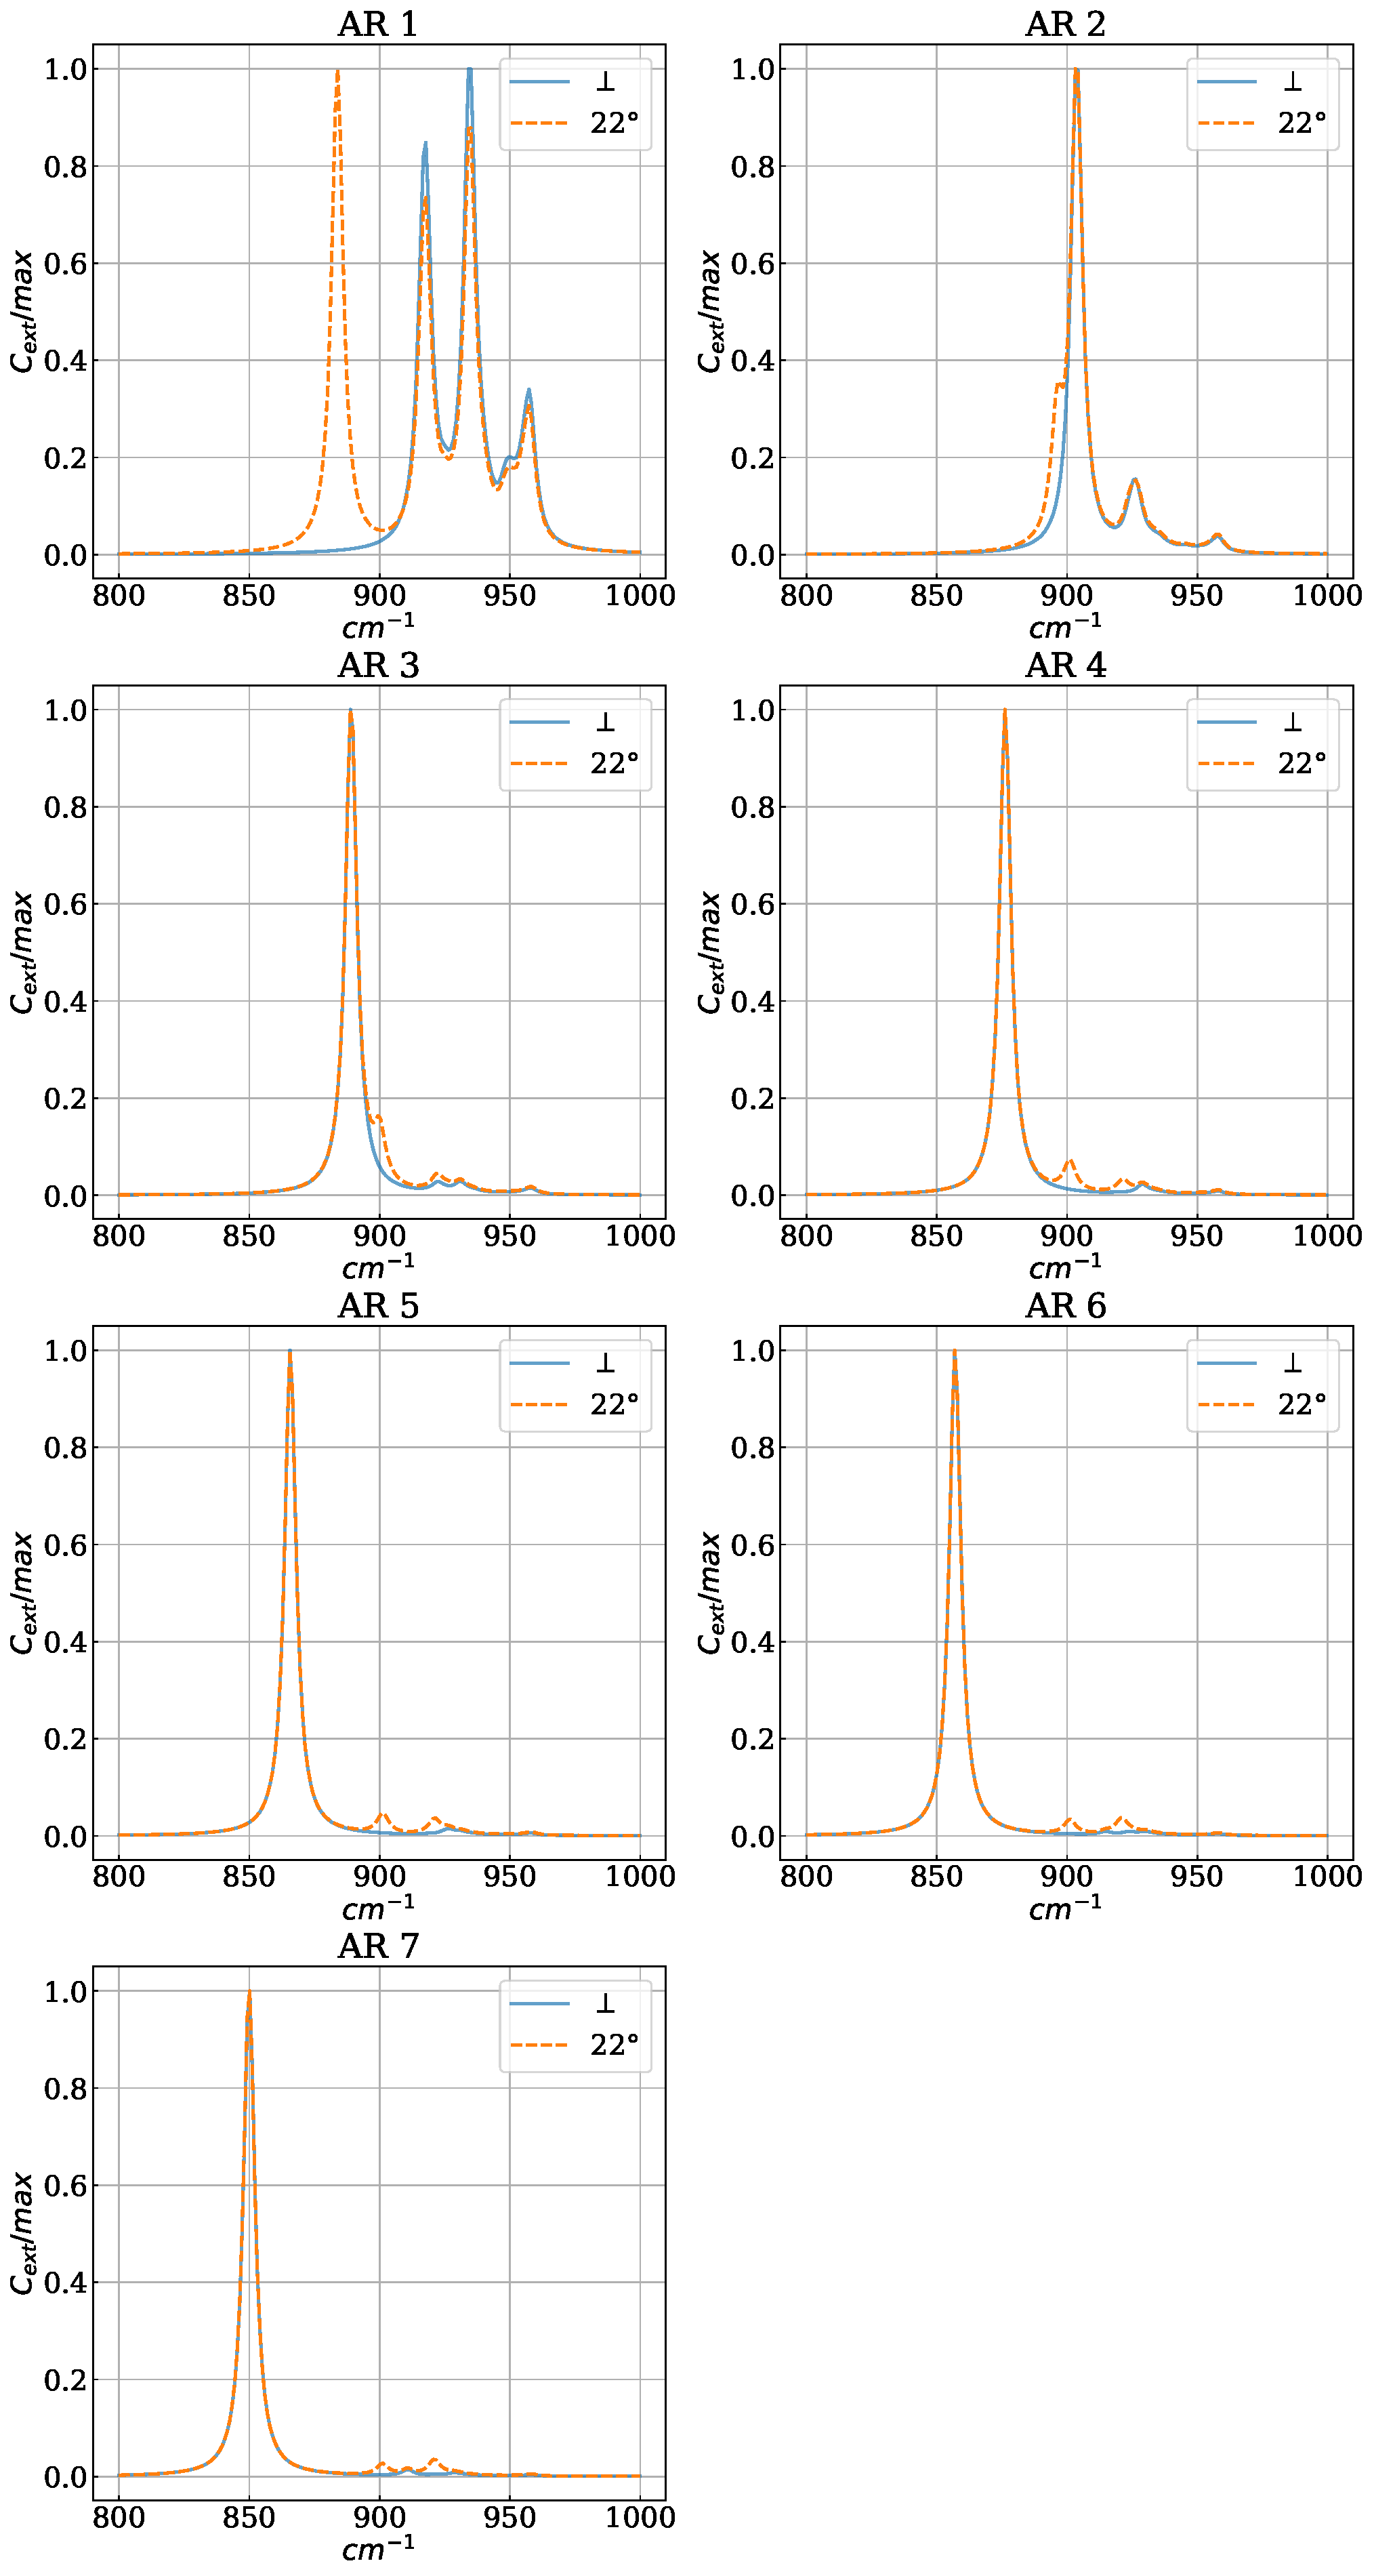
\includegraphics[width=0.85\textwidth]{AR_22_vs_norm.pdf} 
    \caption{ Extinction cross section across wave number for SiC pillars of multiple Aspect ratios. 
             (H=950 nm, W=400nm, L=400-2800 (AR=1-7))
            Normalized by maximum extinction cross section as a function of wave number,
            for a pillar orientation such that the electric field is parallel polarized 
            (I HAVE TO EXPLAIN THIS BETTER, IT ALIGNS WITH THE LENGTH OF THE PILLAR). 
            We present the results for normal incidence and 22 degrees incidence, 
            for different aspect ratios (AR)
            }
    \label{fig:AR_22_vs_norm}
 \end{figure}


\begin{table}
    \begin{center}
      \caption{Wavelength at which peaks happen for different aspect ratios, for runs where the electric
      field is parallel to the length (L) of the pillar. We have normal incidence and 22 degrees.}
      \label{tab:table1}
      \begin{tabular}{c c c c c c c c}
        \textbf{AR} \\
        \hline
        \multirow{2}{*}{1} & $\perp$ & \textbf{917.73} & 934.092 & 949.604 & 957.325 \\ % <-- Combining 2 rows with arbitrary with (*) and content 12
        & 22$^{\circ}$ & 883.926 & \textbf{917.73} & 935.052 & 949.604 & 957.325 \\ % <-- Content of first column omitted.
        \hline
        \multirow{2}{*}{2} & $\perp$ & \textbf{903.233} & 926.395 & 944.762 & 958.242 \\ % <-- Combining 2 rows with arbitrary with (*) and content 12
        & 22$^{\circ}$ & 896.517 & \textbf{903.233} & 926.395 & 944.762 & 958.242 \\ % <-- Content of first column omitted.
        \hline
        \multirow{2}{*}{3} & $\perp$ & \textbf{888.793} & 922.552 & 931.223 & 948.613 & 958.242 \\ % <-- Combining 2 rows with arbitrary with (*) and content 12
        & 22$^{\circ}$ & \textbf{888.793} & 899.418 & 922.552 & 931.223 & 958.242 \\ % <-- Content of first column omitted.
        \hline
        \multirow{2}{*}{4} & $\perp$ & \textbf{876.186} & 929.32 & 946.639 & 958.242 \\ % <-- Combining 2 rows with arbitrary with (*) and content 12
        & 22$^{\circ}$ & \textbf{876.186} & 901.281 & 921.618 & 929.32 & 945.745 & 958.242 \\ % <-- Content of first column omitted.
        \hline
        \multirow{2}{*}{5} & $\perp$ & \textbf{865.576} & 926.395 & 945.745 & 958.242 \\ % <-- Combining 2 rows with arbitrary with (*) and content 12
        & 22$^{\circ}$ & \textbf{865.576} & 901.281 & 921.618 & 958.242 \\ % <-- Content of first column omitted.
        \hline
        \multirow{2}{*}{6} & $\perp$ &  \textbf{856.904} & 914.793 & 923.489 & 929.32 & 946.639 & 958.242\\ % <-- Combining 2 rows with arbitrary with (*) and content 12
        & 22$^{\circ}$ & \textbf{856.904} & 901.281 & 920.6 & 958.242\\ % <-- Content of first column omitted.
        \hline
        \multirow{2}{*}{7} & $\perp$ &  \textbf{850.134} & 910.963 & 921.618 & 928.372 & 946.639 & 958.242 \\ % <-- Combining 2 rows with arbitrary with (*) and content 12
        & 22$^{\circ}$ & \textbf{850.134} & 901.281 & 910.963 & 920.6 & 958.242\\ % <-- Content of first column omitted.
        \hline

      \end{tabular}
    \end{center}
  \end{table}


In other words, we choose the lower mode (lower wavenumber) from the normal 
incidence cases.

Our simulations differ on the method and we do not have a substrate included. The black curve on 
Ellis et al \cite{ellis2016} represents the resonance positions for the $E_{100}$ mode for the different 
aspect ratios when the pillar are separated by a 5000 nm gap. The simulations performed with \pygbe 
consist of one isolated pillar.

\begin{figure}
    \centering
    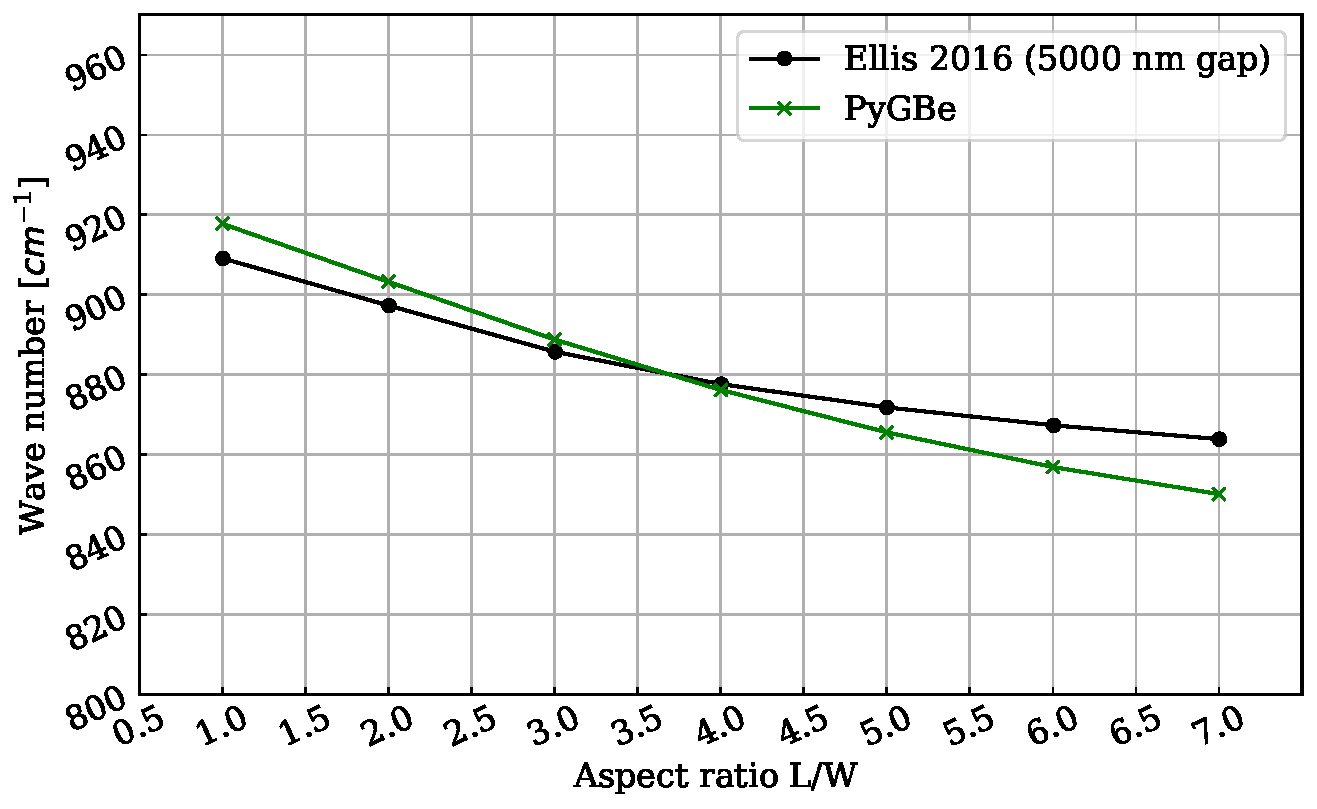
\includegraphics[width=0.85\textwidth]{AR_rep_FS4_Ellis2016.pdf} 
    \caption{Replication of figure S4 of supplementary material of Ellis 2016}
    \label{fig:rep_FS4_ellis}
 \end{figure}

 If we calculate de relative percentage error for each of these points we get:
 
 \begin{table}
    \centering
    \caption{\label{table:err_AR} Percentage error for different aspect ratios.} 
    \begin{tabular}{c c}
    \hline%\toprule
    ARR & \% error \\
    \hline%\midrule
     $1$ & $0.95$ \\
     $2$ & $0.67$ \\
     $3$ & $0.35$ \\
     $4$ & $0.16$ \\
     $5$ & $0.72$ \\
     $6$ & $1.20$ \\
     $7$ & $1.59$ \\
    \hline%\bottomrule
    \end{tabular}
\end{table}


\pygbe AR=4 attempt of validation Figure 2a (see Figure \ref{fig:pygbe_vs_exp_2a})

\begin{figure}
    \centering
    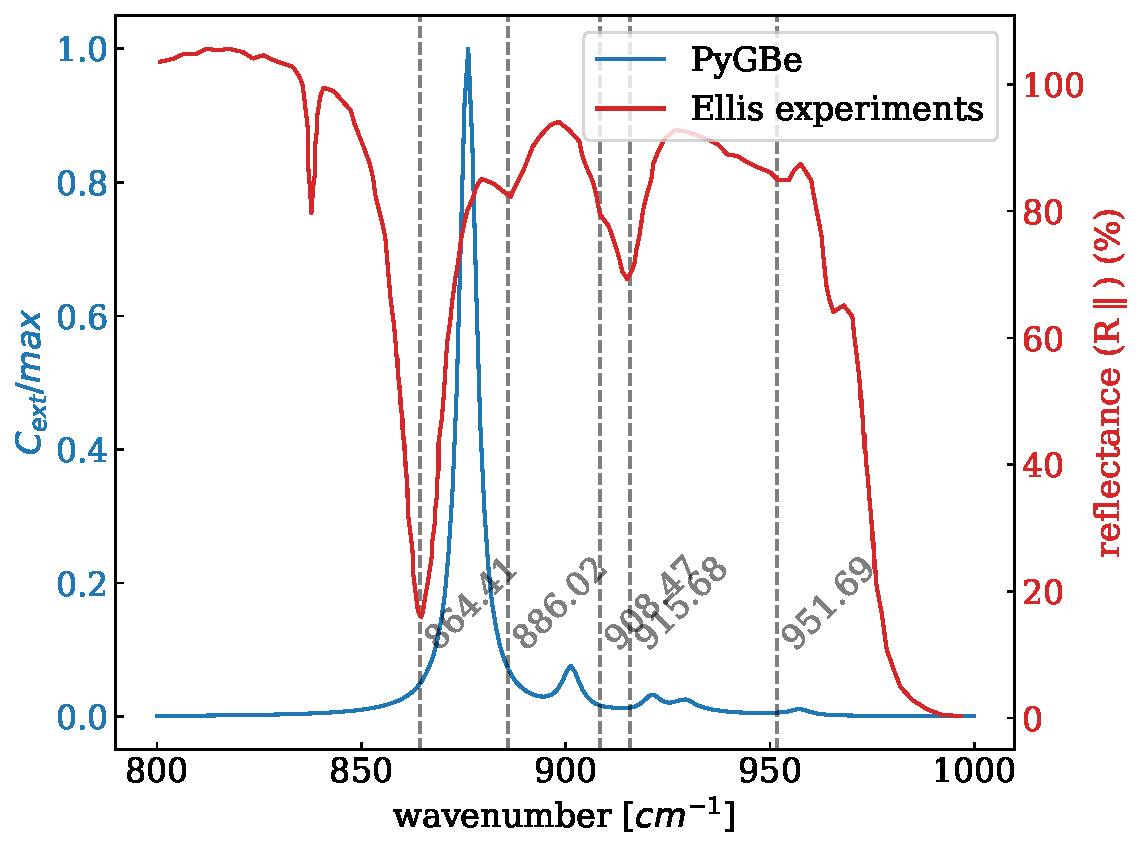
\includegraphics[width=0.85\textwidth]{pygbe_vs_exp_fig2a_Ellis.pdf} 
    \caption{\pygbe vs experiments, figure 2a of Ellis 2016. Ellis et al 
    has near field interaction in its experiments. Ellis data was digitized
    with web digitizer.}
    \label{fig:pygbe_vs_exp_2a}
 \end{figure}

First order approximation to achieve validation. In our code we do not have near 
field interaction. From Figure S4 in supplementary material of Ellis et al. We know that 
for the first mode ($E_{100}$) the difference between interaction and no interaction is 
12.17 $cm^{-1}$ (obtained from digitized data). If we use this as a first order approximation,
we can subtract that value from our curve, and the results are in Figure \ref{fig:val_2a}

\begin{figure}
    \centering
    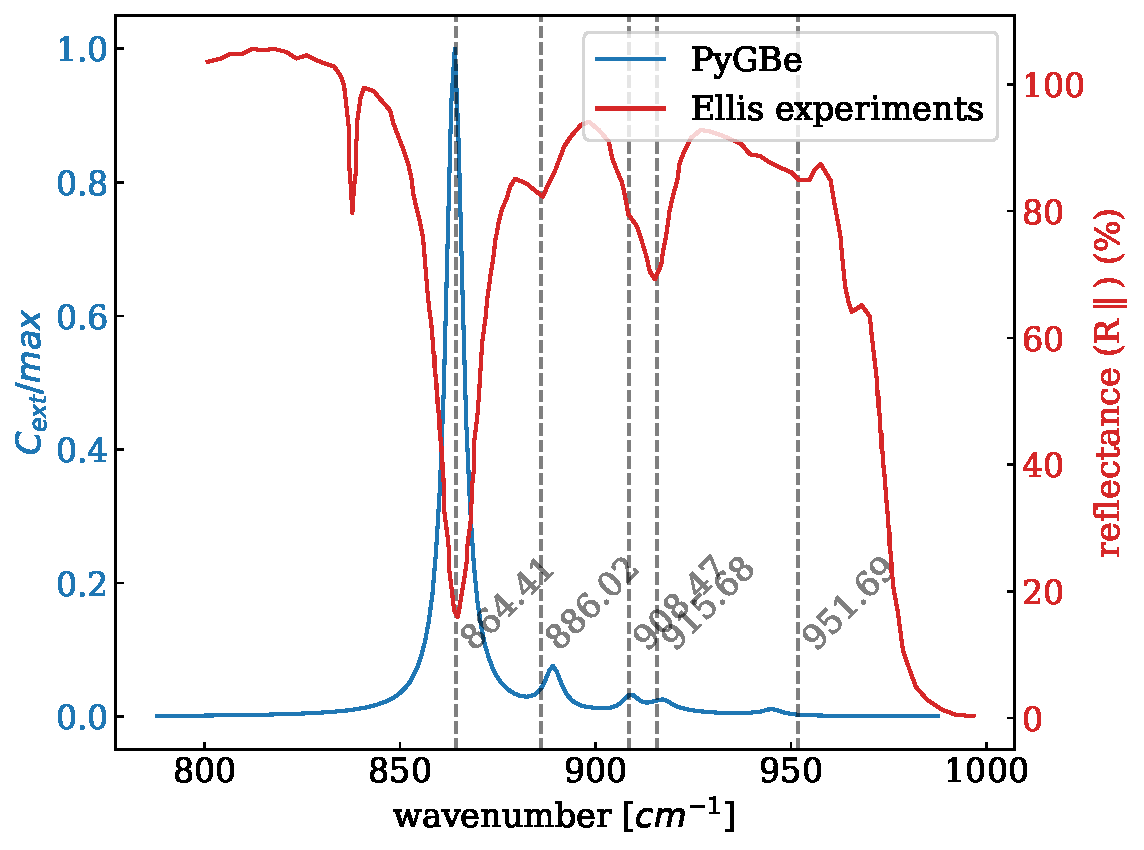
\includegraphics[width=0.85\textwidth]{validation_FOA_fig2a_Ellis.pdf} 
    \caption{Validation against experiments in figure 2a of Ellis 2016, using first order approximation}
    \label{fig:val_2a}
 \end{figure}

If we use the same approximation and compare the results with Ellis simulations on
Figure 2 of their paper (green curve) we get (see Figure \ref{fig:rep_2a})

\begin{figure}
    \centering
    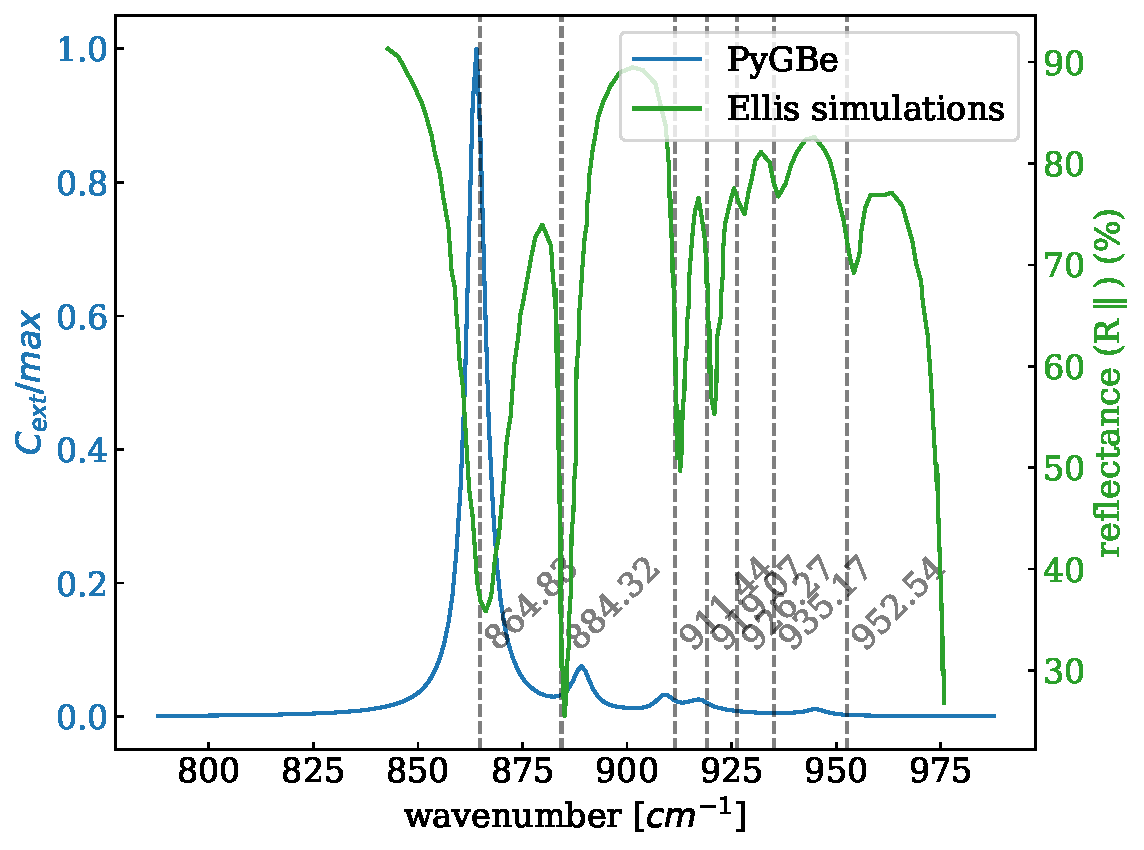
\includegraphics[width=0.85\textwidth]{replication_FOA_fig2a_Ellis.pdf} 
    \caption{Replication of simulations in figure 2a of Ellis 2016, using first
     order approximation}
    \label{fig:rep_2a}
 \end{figure}